\section{System Description}\label{sec:system}

\dReach{} asks the user to provide one input file and two parameters as follows: 
\begin{itemize}
\item The input file that describes the hybrid system and reachability properties in question, with a grammar described in Section~\ref{}. 
\item A bound on the number of mode changes. 
\item A numerical error bound $\delta$, as explained in Section~\ref{}.
\end{itemize}

The tool uses a concise logical encoding that generates a logic formula, which involves existential quatification as well as universal quantification on the time variables. The encoding is compact, always linear in the size of the input file and the number of mode changes. It then makes iterative calls to the underlying solver \dReal{}~\cite{DBLP:conf/cade/GaoKC13} to decide the reachability properties, and generate a visualization of the counterexample if one can be found. Figure~\ref{fig:system-description} illustrates the architecture of
\dReach{}. 

\begin{figure}[!h]
  \centering
  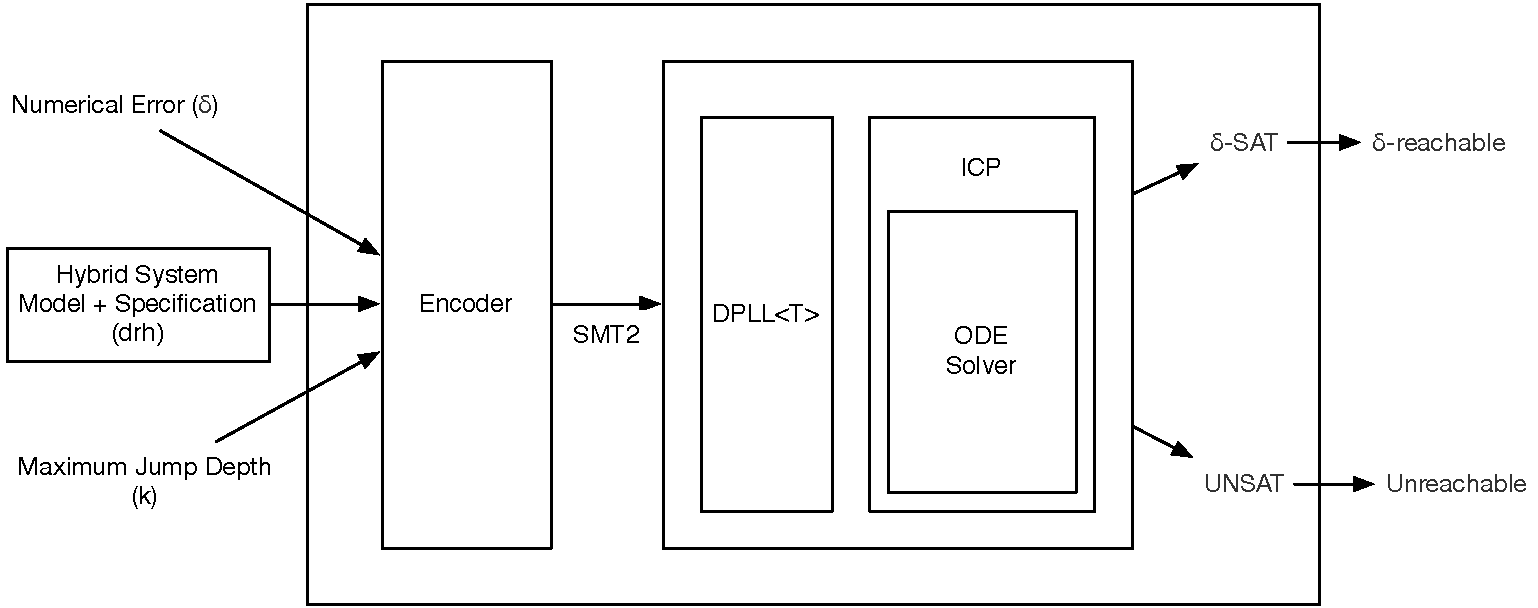
\includegraphics[width=\textwidth]{images/dreach_archi}
  \caption{Architecture of \dReach{}: It consists of an bounded
    model-checking module and an SMT solver, \dReal{}. In the first
    phase, the Encoder module translates an input hybrid system into a
    logic formula. In the second phase, an
    SMT solver, \dReal{}, solves the encoded $\delta$-reachability
    problem using a solving framework that combines DPLL(T), Interval Constraint Propagation, and reliable (interval-based) numerical integration. 
  }  
  \label{fig:system-description}
\end{figure}



%%% Local Variables:
%%% mode: latex
%%% TeX-master: "main"
%%% End:
